\documentclass[../main.tex]{subfiles}
\begin{document}

\section{Topological Artist Model}
\label{sec:tam}

As discussed in the introduction, visualization is generally defined as structure preserving maps from data to graphic representation. In order to formalize this statement, we describe the connectivity of the records using topology and define the structure on the components in terms of the monoid actions on the component types. By formalizing structure in this way, we can evaluate the extent to which a visualization preserves the structure of the data it is representing and build structure preserving visualization tools. We introduce the notion of an artist $\mathscr{\vartist}$ as a structure preserving map from data $\mathscr{\dtotal}$ to $\mathscr{\gtotal}$
\begin{equation}
    \label{eq:artist}
    \mathscr{\vartist}: \mathscr{\dtotal} \rightarrow \mathscr{\gtotal}
\end{equation}

We model the data $\mathscr{\dtotal}$, graphic $\mathscr{\gtotal}$, and intermediate visual encoding $\mathscr{\vtotal}$ stages of visualization as topological structures that encapsulate types of variables and continuity; by doing so we can develop implementations that keep track of both in ways that let us distribute computation while still allowing assembly and dynamic update of the graphic. To explain which structure the artist is preserving, we first describe how we model data(\ref{sec:data}), graphics(\ref{sec:graphic}), and intermediate visual characteristics (\ref{sec:artist}) as fiber bundles. We then discuss the equivariant maps between data and visual characteristics (\ref{sec:artist_nu}) and visual characteristics and graphics (\ref{sec:artist_q}) that make up the artist.
\note{xi should maybe be moved down to artist but is more readable in graphics}

\subsection{Data Space \dtotal}
\label{sec:data}
Building on Butler's proposal of using fiber bundles as a common data representation format for visualization data\cite{butlerVectorBundleClassesForm1992, butlerVisualizationModelBased1989}, a fiber bundle is a tuple $(\dtotal,\,\dbase,\,\pi ,\,\dfiber)$ defined by the projection map $\pi$
\begin{equation}
    \label{eq:fiber_bundle}
    \begin{tikzcd}
        \dfiber \arrow[r, hook] & \dtotal \arrow[r, "\pi"] & \dbase
    \end{tikzcd}
\end{equation}

that binds the components of the data in \dfiber\ to the continuity represented in \dbase. The fiber bundle models the properties of data component types \dfiber\ (\ref{sec:data_fiber}), the continuity of records \dbase\ (\ref{sec:data_base}), the collections of records \dsection\ (\ref{sec:data_section}), and the space \dtotal\ of all possible datasets with these components and continuity. 

By definition fiber bundles are locally trivial\cite{spanier1989algebraic,LocallyTrivialFibre}, meaning that over a localized neighborhood we can dispense with extra structure on \dtotal\ and focus on the components and continuity. We use fiber bundles as the data model because they are inclusive enough to express all the types of data described in section~\ref{sec:intro_data}. 

\subsubsection{Variables: Fiber Space \dfiber}
\label{sec:data_fiber}
To formalize the structure of the data components, we use notation introduced by Spivak \cite{spivakSIMPLICIALDATABASES} that binds the components of the fiber to variable names and types. Spivak constructs a set \ftotal\ that is the disjoint union of all possible objects of types $\{\ftype_0, \ldots, \ftype_n\} \in \ftypes$, where \ftypes\ are the data types of the variables in the dataset. He then defines the single variable set \fttype\ 
\begin{equation}
    \label{eq:data_types}
    \begin{tikzcd}
        \fttype \arrow[r] \arrow[d, "\pi_{\fsection}"'] & \ftotal \arrow[d, "\pi"] \\
        \fnames \arrow[r, "\fsection"']                          & \ftypes       
    \end{tikzcd}
\end{equation}
which is \ftotal\ restricted to objects of type \ftype\ bound to variable name \fname. Given \fsection, the fiber for a one variable dataset is
\begin{equation}
    \dfiber = \ftotal_{\fsection(\fname)} = \ftotal_{\ftype} 
\end{equation}
where \fsection\ is the schema binding variable name \fname\ to its datatype \ftype. A dataset with multiple variables has a fiber that is the cartesian cross product of $\ftotal_{\fsection}$ applied to all the columns:
\begin{equation}
F = \ftotal_{\ftype_1}\times \ldots \ftotal_{\ftype_i} \ldots\times \ftotal_{\ftype_n}
\end{equation}
which is equivalent to 
\begin{equation}
    \dfiber= \dfiber_{0} \times \ldots \times \dfiber_{i}\times\ldots\times \dfiber_{n}
\end{equation}

which allows us to decouple \dfiber\ into components $\dfiber_i$. 

\begin{figure}[H]
    \begin{subfigure}{.5\textwidth}
        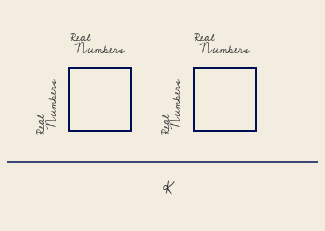
\includegraphics[width=\textwidth]{figures/math/temp_2f.png}
        \caption{}
        \label{fig:fiber_example_plane}
    \end{subfigure}
    \begin{subfigure}{.5\textwidth}
        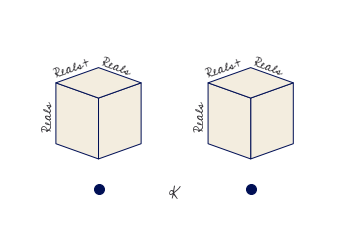
\includegraphics[width=\textwidth]{figures/math/temp_3f.png}
        \caption{}
        \label{fig:fiber_example_cube}
    \end{subfigure}
    \caption{These two datasets have the same base space \dbase\, but figure~\ref{fig:fiber_example_plane} has fiber  $\dfiber=\reals\times\reals$ which is (time, temperature) while figure~\ref{fig:fiber_example_cube} has fiber $\realsp\times\reals^2$ which is (time, wind=(speed, direction))}
    \label{fig:data_fiber_example}
\end{figure}

For example, the data in figure~\ref{fig:fiber_example_plane} is a pair of times and \textdegree K temperature measurements taken at those times. Time is a positive number of type \texttt{datetime} which can be resolved to floats $\ftotal_{\texttt{datetime}}= \reals$. Temperature values are real positive numbers $\ftotal_{\texttt{float}} = \realsp$. The fiber is 
\begin{equation}
    \ftotal =  \reals \times \realsp 
\end{equation} 
where the first component $F_0$ is the set of values specified by $(\fname_0=time,\, \ftype_0=\texttt{datetime},\, \fttype=\reals)$ and $F_1$ is specified by $(\fname_1=temperature,\, \ftype_1=\texttt{float},\, \fttype=\realsp)$ and is the set of values $\fttype=\realsp$. In figure~\ref{fig:fiber_example_cube}, temperature is replaced with wind. This wind variable is of type \texttt{wind} and has two components speed and direction $\{(s,d) \in \reals^{2} \mid  0\leq s,\, 0 \leq d \leq 360\}$ . Therefore, the fiber is 
\begin{equation}
    \dfiber = \realsp \times \reals^{2}
\end{equation} 
such that $F_1$ is specified by $(\fname_1 = wind,\, \ftype_1=\texttt{wind},\, \fttype=\reals^{2})$.  As illustrated in figure~\ref{fig:data}, Spivak's framework provides a consistent way to describe potentially complex components of the input data. 

\subsubsection{Measurement Scales: Monoid Actions}
\label{sec:data_monoid}
Implementing expressive visual encodings requires formally describing the structure on the components of the fiber, which we define as the action of a monoid on the component. While structure on a set of values is often described algebraically as operations or through the actions of a group, for example Steven's scales \cite{stevensTheoryScalesMeasurement1946}, we generalize to monoids to support more component types. Monoids are also commonly found in functional programming because they specify compositions of transformations \cite{yorgeyMonoidsThemeVariations, stievenMonadJustMonoid2020}. 

A monoid \cite{Monoid2021} $\monoid$ is a set with an associative binary operator $\ast:\monoid \times \monoid\rightarrow \monoid$. A monoid has an identity element $e\in \monoid$ such that $e\ast a= a \ast e = a$ for all $a \in \monoid$. As defined on a component of \dfiber, a left monoid action \cite{SemigroupAction2021,ActionNLab} of $\monoid_i$ is a set $\dfiber_i$ with an action $\bullet: \monoid\times \dfiber_i \rightarrow \dfiber_i$ with the properties:
\begin{align*}
    \textbf{associativity}\;& \text{for all } f,g \in \monoid_i \text{ and } x\in \dfiber_i,\, f\bullet(g\bullet x) = (f\ast g) \bullet x\\
    \textbf{identity}\;& \text{for all } x\in \dfiber_i, e\in \monoid_i,\,  e\bullet x = x 
\end{align*}
As with the fiber \dfiber\, the total monoid space \monoid\ is the cartesian product
\begin{equation}
\monoid= \monoid_{0} \times \ldots \times \monoid_{i}\times \ldots \times\ldots \monoid_{n}
\end{equation}
of each monoid $\monoid_{i}$ on $\dfiber_{i}$.  The monoid is also added to the specification of the fiber $(\fname_i,\, \ftype_i,\, \fttype\, \monoid_i)$

Steven's described the measurement scales\cite{stevensTheoryScalesMeasurement1946,leaFormalizationMeasurementScale} in terms of the monoid actions on the measurements: nominal data is permutable, ordinal data is monotonic, interval data is translatable, and ratio data is scalable \cite{weissteinSimilarityTransformation}. For example, given the interval scale fiber component $(\fname=temperature,\, \ftype=\texttt{float},\,\fttype=\reals)$:
\begin{itemize}
    \item monoid operator addition $\ast = +$
    \item monoid operations: $f: x\mapsto x + 1 $, $g: x\mapsto x + 2  $
    \item monoid action operator composition $\bullet = \circ$
\end{itemize}
then the translation monoid actions on temperature satisfy the condition
\begin{equation}
    \begin{tikzcd}
        \reals \arrow[rd, "(x+ 1\degree)\circ(x+2\degree)"] \arrow[d, "x+ 1\degree"'] &            \\
        \reals \arrow[r, "x+ 2\degree"']                                   & \reals
    \end{tikzcd}
\end{equation}
where $1\degree$ and $2\degree$ are valid distances between two temperatures $x$. 

While many component types will be one of the measurement scale types, we generalize to monoids specifically for the case of partially ordered set. Given a set $W=\{mist, \, drizzle, \, rain \}$, then the map $f: W\rightarrow W$ defined by 
\begin{enumerate}
    \item $f(rain) = drizzle$,
    \item  $f(drizzle) = mist$ 
    \item $f(mist) = mist$
\end{enumerate}
is order preserving such that $mist \leq drizzle \leq rain$ but has no inverse since $drizzle$ and $mist$ go to the same value $mist$. Therefore order preserving maps do not form a group, and instead we generalize to monoids to support partial order component types. Defining the monoid actions on the components serves as the basis for identifying the invariance\cite{kindlmann2014algebraic} that must be preserved in the visual representation of the component. 

\subsubsection{Continuity: Base Space $K$} 
\label{sec:data_base}
The base space \dbase\ is way to express the connectivity of the records.  This is assumed in the choice of visualization, for example a line plot implies 1D continuous data and a scatter plot implies discrete records, but an explicit representation allows for verifying that the topology of the graphic representation is equivalent to the topology of the data.  

\begin{figure}[H]
    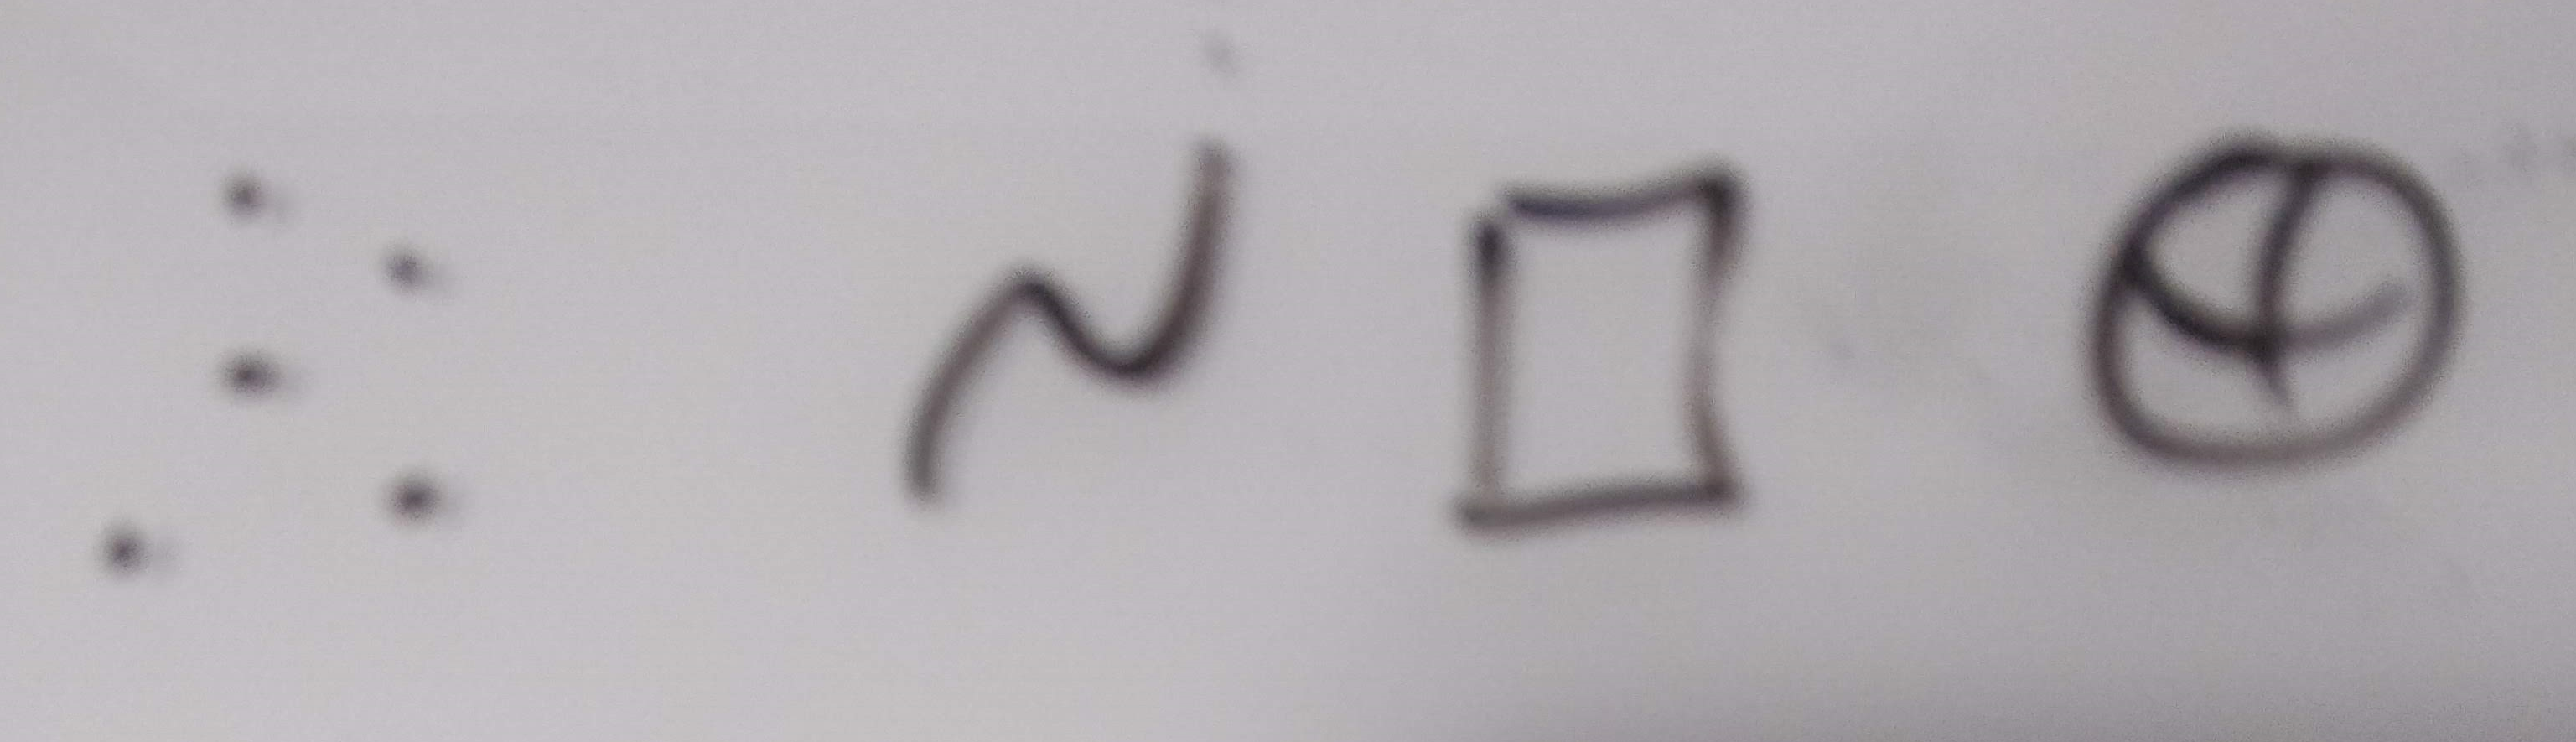
\includegraphics[width=.5\textwidth]{figures/math/k_different_types.png}
    \caption{The topological base space \dbase\ encodes the connectivity of the data space, for example if the data is independent points or a map or on a sphere}
    \label{fig:base_space_types}
\end{figure}
As illustrated in figure~\ref{fig:base_space_types}, \dbase\ is akin to an indexing space into \dtotal\ that describes the structure of \dtotal.  \dbase\ can have any number of dimensions and can be continuous or discrete. 

\begin{figure}[H]
    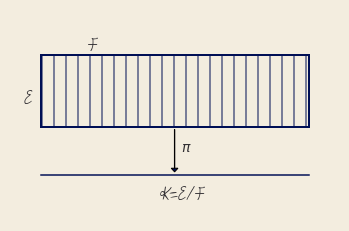
\includegraphics[width=.5\linewidth]{figures/math/k_qspace.png}
    \caption{The base space \dtotal\ is divided into fiber segments \dfiber. The base space \dbase\ acts as an index into the records in the fibers.
    \note{this figure might be good all the way up top to lay out the components of fb}}
    \label{fig:base_space_div}
\end{figure}

Formally \dbase\ is the quotient space \cite{QuotientSpaceTopology2020} of \dtotal\, meaning it is the finest space\cite{aurouxMath131Introduction} such that every $\dbasepoint \in \dbase$ has a corresponding fiber $\dfiber_k$\cite{QuotientSpaceTopology2020}. In figure~\ref{fig:base_space_div}, \dtotal\ is a rectangle divided by vertical fibers \dfiber, so the minimal \dbase\ for which there is always a mapping $\pi: \dtotal\rightarrow \dbase$ is the line. 

As with fibers and monoids, we can decompose the total space into components $\pi:\dtotal_i\rightarrow \dbase$ where
\begin{equation}
    \pi:\dtotal_1\oplus\ldots\oplus \dtotal_i \oplus\ldots \oplus \dtotal_n \rightarrow \dbase
\end{equation}

which is a decomposition of \dfiber. The \dbase\ remains the same because the connectivity of records does not change just because there are fewer elements in each record.
\begin{figure}[ht!]
    \begin{subfigure}{.5\textwidth}
        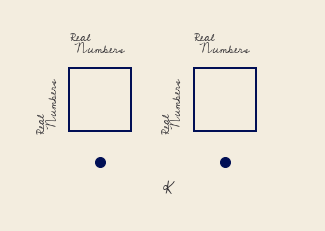
\includegraphics[width=\textwidth]{figures/math/temp_1k.png}
        %% add box around neighboring P and Map
        \caption{}
        \label{fig:base_example_discrete}
    \end{subfigure}
    \begin{subfigure}{.5\textwidth}
        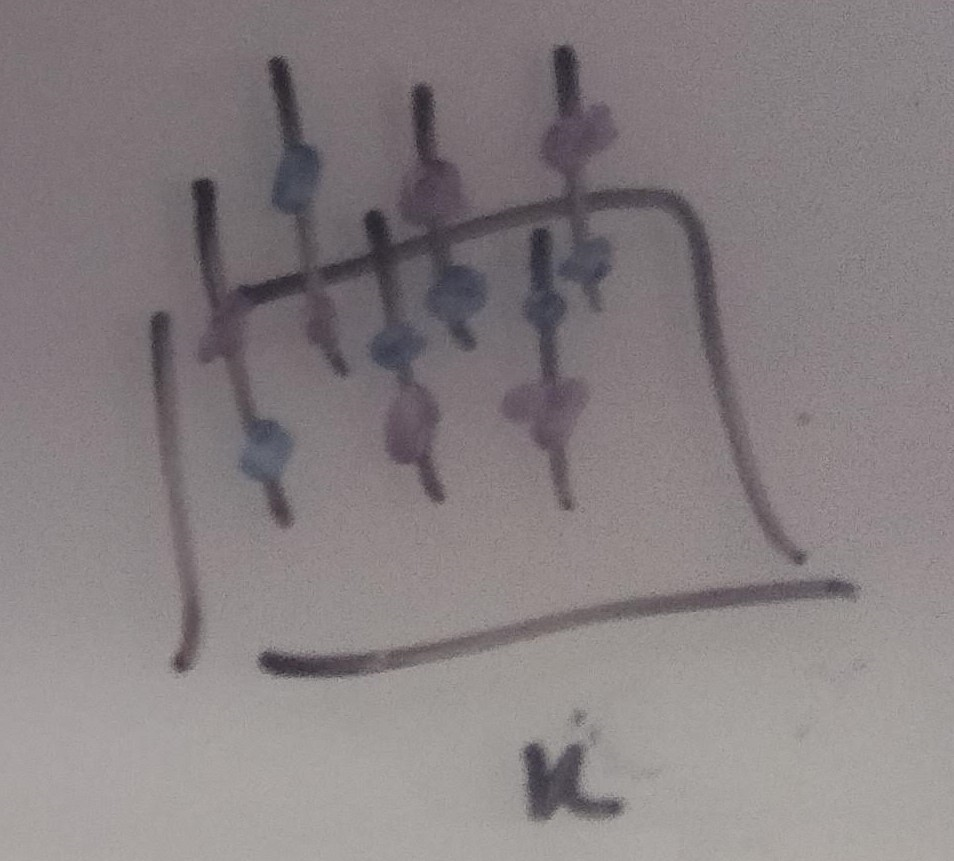
\includegraphics[width=\textwidth]{figures/math/temp_2k.png}
        \caption{}
        \label{fig:base_example_continuous}
    \end{subfigure}
    \caption{These two datasets have the same (time, temperature) fiber. In figure~\ref{fig:base_example_line} the total space \dtotal\ is discrete over points $\dbasepoint \in \dbase$, meaning the records in the fiber are also discrete. In figure~\ref{fig:base_example_plane} \dtotal\ lies over the continuous interval \dbase, meaning the records in the fiber are sampled from a continuous space. 
    \note{revamp figure: F=Plane, k1 = dots, k2=line}}
    \label{fig:base_example}
\end{figure}

The datasets in figure~\ref{fig:base_example} have the same fiber of (temperature, time). In figure~\ref{fig:base_example_discrete} the fibers lie over discrete \dbase\ such that the records in the datasets in the fiber bundles are discrete. The same fiber in figure~\ref{fig:base_example_continuous} lies over a continuous interval \dbase such that the records are samples from a continuous function defined on \dbase. By encoding this continuity in the model as \dbase\, the data model now explicitly carries information about its structure such that the implicit assumptions of the visualization algorithms are now explicit. This in turn allows for building algorithms that can work with distributed or streaming data, since it has a common data access interface with a promise that the data exists. 

\subsubsection{Data: Sections \dsection}
\label{sec:data_section}
A set of records is a section $\dsection: \dbase\rightarrow \dtotal$ of the fiber bundle. For example, in the special case of a table \cite{spivakSIMPLICIALDATABASES}, \dbase\ is a set of row ids, \dfiber\ is the columns, and the section \dsection\ returns the record at a given key in \dbase. In general, for any fiber bundle, there is always a map
\begin{equation}
    \begin{tikzcd}
        \dfiber \arrow[r, hook] & \dtotal \arrow[d, "\pi"'] \\
                          & \dbase \arrow[u, "\dsection"', bend right]
    \end{tikzcd}
\end{equation}
 such that $\pi(\dsection(\dbasepoint)) = \dbasepoint$. There can be many sections \dsection\ and the space of all global sections is $\Gamma(\dtotal)$. Assuming a trivial fiber bundle $\dtotal = \dbase \times \dfiber$, the section is 
\begin{equation}
    \label{eq:section_return}
    \dsection(\dbasepoint) = (\dbasepoint, (g_{\dfiber_{0}}(\dbasepoint), \ldots, g_{\dfiber_{n}}(\dbasepoint)))
\end{equation}
where $g: \dbase \rightarrow \dfiber$ is the index function into the fiber. This formulation of the section also holds on locally trivial sections of a non-trivial fiber bundle. Because we can decompose the bundle and the fiber, we can formulate $\dsection$ as 
\begin{align}
\dsection= (\dsection_0,\ldots, \dsection_i, \dots, \dsection_n) 
\end{align}
where each section $\dsection_i$ is a variable or set of variables. 

\begin{figure}[H]
    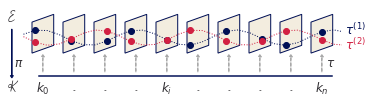
\includegraphics[width=.5\linewidth]{figures/math/fiberbundle.png}
    \caption{ Fiber (time, temperature) with an interval \dbase\ basespace. The sections $\dsection_i$ and $\dsection_j$ are constrained such that the time variable must be monotonic, which means each section is a timeseries of temperature values. They are included in the global set of sections  $\dsection_1, \dsection_2 \in \Gamma(\dtotal)$}
    \label{fig:data_sections}
\end{figure}

In the example in figure~\ref{fig:data_sections}, the fiber is $(time, \, temperature)$ as described in figure~\ref{fig:data_fiber_example} and the base space is the interval \dbase. The section $\dsection_i$ resolves to a series of monotonically increasing in time records of (time, temperature) values. Section $\dsection_j$ returns a different timeseries of (time, temperature) values. Both sections are included in the global set of sections $\dsection_i, \dsection_j \in \Gamma(\dtotal)$.

The section can be any instance of a data container, for example a numpy array\cite{harris2020array}, a pandas series or dataframe\cite{jeff_reback_2020_3715232}, or an xarray\cite{hoyer2017xarray}. A univariate numpy array that stores an image is a section of a fiber bundle where \dbase\ is a 2D continuous plane and the \dfiber\ is $(\reals^{3}, \reals, \reals)$ where $\reals^3$ is color, and the other two components are the x and y positions of the sampled data in the image. A series could store the values of $\dsection_i$ and a second series could be  $dsection_j$. We could also fatten the fiber to hold two temperature series, such that a section would be an instance of a dataframe with a time column and two temperature columns. While the series and dataframe explicitly have a time index column, they are components in our model and the index is always assumed to be random keys. An instance of an xarray would also be a \dsection\, for example if the data is a temperature field than the \dbase\ could be a continuous volume and the components would be the temperature and the time, latitude, and longitude the measurements were sampled at. As with the dataframe, the semantic index labels are considered components and the indicies are instead assumed to be random. A section can also be an instance of a distributed data container, such as a dask array \cite{rocklinDaskParallelComputation2015}. As with the other containers, \dbase\ and \dfiber\ are defined in terms of the index and dtypes of the components of the array. The section can remain curried until render since the model is functional, in keeping with dasks compute graph architecture. Our model provides a common interface to these widely used data containers without sacrificing the semantic structure embedded in each container.

\subsubsection{Sheaf and Stalk}
\label{sec:data_sheaf_stalk}
To support working with a subset of data, we can take the sheaf $\mathcal{O}(\dtotal)$ as input into the artist. \dtotal\ restricted over a small enough neighborhood $U \subset \dbase$ is a locally trivial bundle over $U$\cite{LocallyTrivialFibre}. The sheaf $O(\dtotal)$ is the localized section of fibers $\iota^*\dsection: U \rightarrow \iota^*\dtotal$

\begin{equation}
    \label{eq:sheaf}
    \begin{tikzcd}
        \iota^*\dtotal \arrow[d, "\pi"']           & \dtotal \arrow[d, "\pi"'] \arrow[l, "\iota^*"']         \\
        U \arrow[u, "\iota^*\dsection"', bend right] & \dbase \arrow[u, "\dsection"', bend right] \arrow[l, "\iota"']
    \end{tikzcd}
\end{equation}
pulled back over the neighborhood $U$ via the inclusion map $\iota: U \rightarrow \dbase$. The localized section is the germ $\xi^*\dsection$. The neighborhood of points $\dbasepoint_i$ surrounding the point \dbasepoint\ the sheaf lies over is the stalk $\mathcal{F}_b$ \cite{StalkSheaf2019,spanier1989algebraic}. 

While \dtotal\ is only the fiber $\dfiber_k$ over a specific \dbasepoint, the stalk includes the local behavior of the section at \dbasepoint\ which can include information about nearby records. In practice, often the only information needed from the stalk is some finite number $n$ of derivatives, which is captured by the jet bundle $\mathcal{J}^n$ \cite{JetBundle2020,musilovaCalculusVariationsJet2016} with $\mathcal{J}^{0}(\dtotal)=\dtotal$. In this work, we at most need $\mathcal{J}^{2}(\dtotal)$ which is the value at \dsection\ and its first and second derivatives. The sheaf facilitates interactions such as zooming or updating the graphic based on zooming data; the jet ensures that the artist only needs a single record on \dbasepoint\ to render a piece of a graphic. This allows for the creation of highly concurrent and possibly distributed artists. 


\subsection{Graphic: \gtotal}
\label{sec:graphic}  
We introduce a graphic bundle to hold the essential information necessary to render a graphical design constructed by the artist. As with the data, we can represent the target graphic as a section \gsection\ of a bundle  $(\gtotal, \gbase, \pi, \gfiber)$. The graphic bundle \gtotal\ consists of a base \gbase (~\ref{sec:graphic_fiber}) that is a thickened form of \dbase\, 
a fiber \gfiber (~\ref{sec:graphic_base}) that is an idealized display space, and sections \gsection (~\ref{sec:graphic_section}) that encode a graphic where the visual characteristics are fully specified.

\subsubsection{Idealized Display \gfiber}
\label{sec:graphic_fiber}
To fully specify the visual characteristics of the image, we construct a fiber \gfiber\ that is an infinite resolution version of the target space. Typically \gtotal\ is trivial and therefore sections can be thought of as mappings into \gfiber. 

In this work, we assume a 2D opaque image $\gfiber=\reals^5$ with elements 
\begin{equation}
(x,\, y,\, r,\, g,\, b) \in \gfiber
\end{equation}
such that a rendered graphic only consists of 2D position and color. To support overplotting and transparency, the fiber could be $\gfiber=\reals^{7}$ such that $(x, y, z, r, g, b, a) \in \gfiber$ specifies the target display. By abstracting the target display space as \gfiber, the model can support different targets, such as a 2D screen or 3D printer. 

\subsubsection{Continuity of the Graphic \gbase} 
\label{sec:graphic_base}
Since we propose that data topology \dbase\ is by some measure preserved in the graphic, we introduce a graphic topology \gbase to encode the carried over structure. These topologies are not always identical because the underlying topology \gbase\ of a graphic may need more dimensions than the data topology \dbase\. In a typical 2D display (ignoring depth), visible elements need to have 2D extent so that for example a scatter marker has an area greater than 0 or a line is not infinitely thin. 

Since \dbase\ with fewer than two dimensions need to be thickened, we define the mapping from graphic \gbase\ to data \dbase 
\begin{equation}
    \begin{tikzcd}
        \dtotal \arrow[d, "\pi"'] & \gtotal \arrow[d, "\pi"'] \\
        \dbase                   & \gbase \arrow[l, "\vindex"']
        \end{tikzcd}
\end{equation}

 as the deformation retraction \cite{RetractionTopology2020} $\vindex: \gbase \rightarrow \dbase$ that goes from a region $\gbasepoint \in \gbase_{\dbasepoint}$ to its associated point $\gbasepoint$, such that when $\vindex(\gbasepoint) = \dbasepoint$,\, $\vindex^*\dsection(\gbasepoint) = \dsection(\gbasepoint)$. While dimensions can be added to \gbase, it retains the same continuity as \dbase.
 
\begin{figure}
    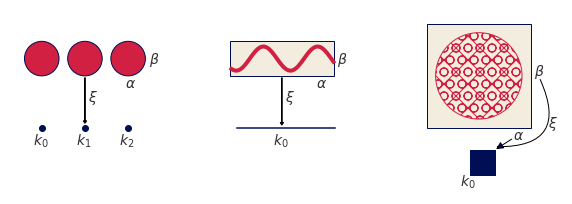
\includegraphics[width=1\textwidth]{figures/math/retraction_maps.png}
    \caption{The scatter and line graphic base spaces have one more dimension of continuity than \dbase\ so that \gbase\ can encode physical aspects of the glyph, such as shape (a circle) or thickness. The heatmap has the same continuity in the graphic \gbase\ as in the data \dbase. \note{add $\alpha, \beta$ coordinates to figures}}
    \label{fig:graphic_retraction_map}
\end{figure}

When \dbase\ is discrete points and the graphic is a scatter plot, each point $\dbasepoint \in \dbase$ corresponds to a 2D disk $\gbase_{\dbasepoint}$ as shown in figure~\ref{fig:graphic_retraction_map}. In the case of 1D continuous data and a line plot, the region \gy\ over a point $\gx_i$ specifies the thickness of the line in \gbase\ for the corresponding \dsection\ on \dbasepoint. The heatmap has the same continuity in data space and graphic space such that no extra dimensions are needed in \gbase. The mapping function \vindex\ provides a way to identify the part of the visual transformation that is specific to the the connectivity of the data rather than the values; for example it is common to flip a matrix when displaying an image. 

\subsubsection{Renderering \gsection}
\label{sec:graphic_section}
\begin{figure}
    \includegraphics[width=\textwidth]{figures/math/graphic_render.png}
    \caption{To render a graphic, a pixel $p$ is selected in the display space, which is defined in the same coordinates as the x and y components in \gfiber\.  The inverse mapping ${\gsection_{xy}}^(p)$ returns a region $\gbase_{p} \subset \gbase$. $\gsection(\gbase_{p})$ returns the list of elements $(x,\,y,\,r,\,g,\,b) \in \gfiber$ that lie over $\gbase_{p}$. The integral over the $(r,\,g,\,b)$ elements is the color of the pixel.}
    \label{fig:graphic_rho_lookup}
\end{figure}

This section describes how we go from a graphical design to a rendered image, where the graphical design is the section $\gsection: \gbase \rightarrow \gtotal$. It is sufficient to sketch out how an arbitrary pixel would be renderer, where a pixel $p$ in a real display corresponds to a region $\gbase_p$ in the idealized display. To determine the color of the pixel, we aggregate the color values over the region via integration. 

For a 2D screen, the pixel is defined as a region $p=\left[y_{top}, y_{bottom}, x_{right}, x_{left}\right]$ of the rendered graphic. Since the x and y in $p$ are in the same coordinate system as the x and y components of \gfiber\,  the inverse map of the bounding box $\gbase_{p} ={\gsection_{xy}}^{-1}(p)$ is a region $\gbase_p \subset \gbase$. To compute the color, we integrate on $\gbase_p$

\begin{align}
    r_p &= \iint\limits_{S_p} \rho_r(s)ds^{2}\\
    g_p &= \iint\limits_{S_p} \rho_g(s)ds^{2}\\
    b_p &= \iint\limits_{S_p} \rho_b(s)ds^{2}
\end{align}

As shown in figure~\ref{fig:graphic_rho_lookup}, a pixel $p$ in the output space is selected and inverse mapped into the corresponding region $\gbase_p \subset \gbase$. This triggers a lookup of the $\gsection$ over the region $\gbase_p$, which yields the set of elements in \gfiber\ that specify the $(r, g, b)$ values corresponding to the region $p$. The color of the pixel is then obtained by taking the integral of $\gsection_{rgb}(\gbase_p)$. In general, \gsection\ is an abstraction of rendering specifications, for example PDF\cite{bienz1993portable}, SVG\cite{quintScalable2003}, or an openGL scene graph\cite{CarsonOpenGL1997} or rendering engines such as cairo\cite{CairographicsOrg} and AGG\cite{AntiGrainGeometry}. Implementation of \gsection\ is out of scope for this work.  

\subsection{Artist}
\label{sec:artist}

The artist is the function that converts data into graphics; its name is taken from the analogous part of Matplotlib\cite{hunterArchitectureOpenSource} that builds visual elements to pass off to the renderer. The artist \vartist\ is a mapping from \dtotal\ padded with data from $\dtotal^{\prime}=\mathcal{J}(\dtotal)$ to a graphic that is a section $\gsection \in \Gamma(\gtotal)$

\begin{equation}
    \label{eq:artist_diagram}
    \begin{tikzcd}
        \dtotal^{\prime} \arrow[r, "\vchannel"] \arrow[rd, "\pi"'] & \vtotal \arrow[d, "\pi"] & \vindex^*\vtotal \arrow[r, "\vmark"] \arrow[d, "\vindex^*\pi"'] \arrow[l, "\vindex^*"'] & \gtotal \arrow[ld, "\pi"] \\
                                              & \dbase                  & \gbase \arrow[l, "\vindex"']                                              &                    
        \end{tikzcd}
\end{equation}

which due to using the jet is point wise such that the input can be $\dsection(\dbasepoint)$. The encoders $\vchannel:\dtotal^{\prime} \rightarrow \vtotal$ converts the data components to visual components(\ref{sec:graphic_base}). The continuity map $\vindex:\gbase \dbase$ then pulls back the visual bundle \votal\ over \gbase (\ref{sec:artist_nu}). Then the assembly function $\vmark: \vtotalpull \rightarrow \gtotal$ composites the fiber components of \vtotalpull\ into a graphic in \gtotal (\ref{sec:artist_q}). This functional decomposition of the visualization artists allows us to specify what are the responsibilities of each function in a fully constrained way. In turn, this allows for building reusable components at each stage of the transformation. 




\subsubsection {Visual Fiber Bundle \vtotal}
We introduce a visual bundle \vtotal\ to store the visual representations the artist needs to composite into a graphic. The visual bundle (\vtotal, \dbase, $\pi$, \vfiber) has section $\vsection: \vtotal \rightarrow \dbase$ that resolves to a visual variable in the fiber \vfiber. The visual bundle \vtotal\ is the latent space of possible parameters of a visualization type, such as a scatter or line plot. We define \vfiber\ in terms of the parameters of a visualization libraries compositing functions; for example table~\ref{tab:mpl_visual_variable_fiber} is a sample of the fiber space for Matplotlib \cite{hunterMatplotlib2DGraphics2007}.

\begin{table}[H]
    \renewcommand{\arraystretch}{2}
    \begin{tabulary}{\textwidth}{|l|L|l|}\hline
     $\bm{\vchannel_{i}}$                      & $\bm{\vsection_{i}}$                                                            & $\bm{codomain(\vchannel_{i})}$  \\ \hline                                              
    position                    & x, y, z, theta, r                                                          & $\mathbb{R}$   \\ \hline
    size                        & linewidth, markersize                                            & $\mathbb{R}^{+}$   \\ \hline
    shape                       & markerstyle                                                      & $\{f_{0}, \ldots, f_{n}\}$ \\ \hline
    color                       & color, facecolor, markerfacecolor, edgecolor  & $\mathbb{R}^{4}$ \\ \hline
    \multirow{2}{*}{texture}    & hatch                                                            & $\mathbb{N}^{10}$\\\cline{2-3}
                                & linestyle                                                        & $(\mathbb{R}, \mathbb{R^+}^{n, n\%2=0})$ \\ \hline              
    \end{tabulary}
    \caption{Some possible components of the fiber \vfiber\ for a visualization function implemented in Matplotlib}
    \label{tab:mpl_visual_variable_fiber}
\end{table}

 A section \vsection is a tuple of visual values that specifies the visual characteristics of a part of the graphic. For example, given a fiber of $\{xpos, ypos, color\}$ one possible section could be  $\{.5, .5, (255, 20,147)\}$. The $codomain(\vchannel_i)$ determines the monoid actions on $\vsection_i$. These fiber components are implicit in the library, by making them explicit as components of the fiber we can build consistent definitions and expectations of how these parameters behave. 

\subsubsection{Visual Encoders \vchannel}
\label{sec:artist_nu}
%% equivariant maps 
\begin{figure}
    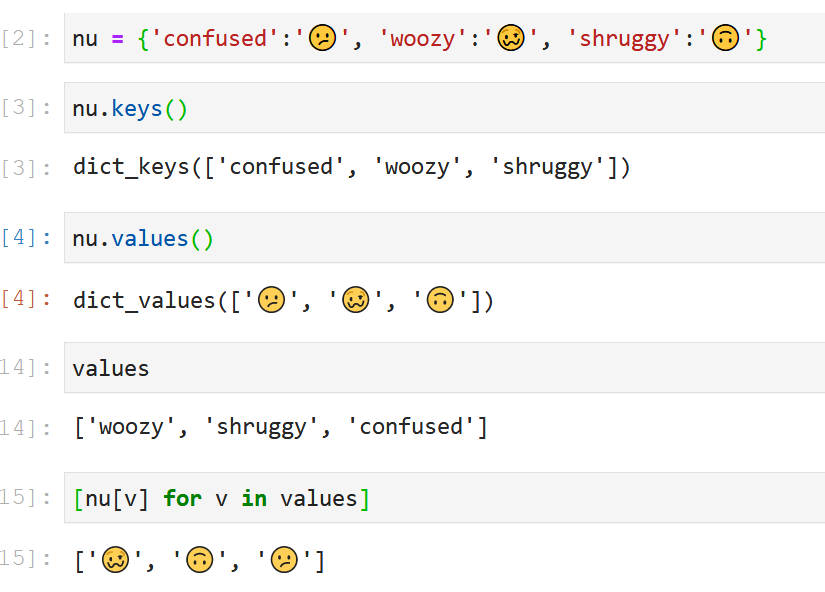
\includegraphics[width=\textwidth]{figures/math/equivariance_nu.png}
    \caption{In this artis, \vchannel\ maps the strings to the emojis. For \vchannel\ to be equivariant, a shuffle in the words should have an equivalent shuffle in the emojies, and a shuffle in the emojies should have an equivalent shuffle in the words.}
    \label{fig:artist_nu}
\end{figure}
As introduced in section~\ref{sec:intro_visual_variables}, there are many ways to encode data visually. We define the visual transformers \vchannel\ as the set of independent conversion functions 
\begin{equation}
    \label{eq:nu_expanded}
    \{\vchannel_{0}, \ldots, \vchannel_{n}\}: \{\dsection_{0}, \ldots, \dsection_{n}\} \mapsto \{\vsection_{0}, \ldots, \vsection_{n}\}
\end{equation}
where $\vchannel_i: \dsection_i \mapsto \vsection_i$ is an equivariant map such that there is a monoid homomorphism from $\dfiber_{i}$ to $vfiber_{i}$. As mentioned in section~\ref{sec:data_monoid}, we choose monoid actions as the basis for equivariance because they define the structure on the fiber components. A validly constructed \vchannel\ is one where the diagram of the monoid transform $m$
\begin{equation}
    \label{eq:nu_categorical}
\begin{tikzcd}
    \dtotal_i \arrow[r] \arrow[r, "\vchannel_i"] \arrow[d, "m_{\delement}"'] & \vtotal_i \arrow[d, "m_{\velement}"] \\
    \dtotal_i \arrow[r, "\vchannel_i"]                           & \vtotal_i               
\end{tikzcd}
\end{equation}
commutes such that $\vchannel_i(m_{\delement}(\dtotal_i)) = m_{\velement}(\vchannel_i(\dtotal_i))$. This equivariance constraint yields guidance on what makes for an invalid transform. For example, the conversion $\vchannel_{i}(x) = .5$ does not commute under translation monoid action $t(x) = x+2$  
\begin{align}
    \vchannel(t(\delement + 2)) & \overset{?}{=} \vchannel(\delement) + \vchannel(2)\\
    .5 &\neq .5 + .5
\end{align}

On the other hand figure~\ref{fig:artist_nu} illustrates a valid \vchannel\ mapping from \textbf{Strings} to symbols. The group action on these sets is permutation, so shuffling the words must have an equivalent shuffle of the symbols they are mapped to. To preserve ordinal and partial order monoid actions, \vchannel\ must be a monotonic function such that given $\delement_1, \delement_2 \in \dtotal_{i}$, $\text{ if } delement_1 \leq \delement_2 \text{ then } \vchannel (\delement_1) \leq \vchannel(\delement_2)$. For interval scale data, \vchannel\ is equivariant under translation monoid actions if $\vchannel (x + c) = \vchannel(x) + \vchannel(c)$. For ratio data, there must be equivalent scaling $ \vchannel(xc) = \vchannel(x)\vchannel(c)$. These constraints can be embedded into our artist such that the \vchannel\ functions are equivariant; they also provide guidance on constructing new equivariant \vchannel\ functions. 

\subsubsection{Graphic Assembler \vmark}
\label{sec:artist_q}
\begin{figure}[H]
    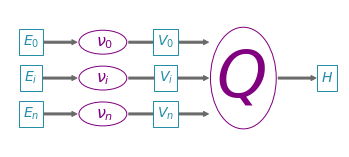
\includegraphics[width=\textwidth]{figures/math/path_of_q}
    \caption{\vchannel\ functions convert data $\dsection_i$ to visual characteristics $\vsection_i$, then \vmark\ assembles $\vsection_i$ into a graphic $\gsection$ such that there is a map \vindex\ preserving the continuity of the data. \gsection\ applied to a region of connected components $\gbase_{\dbasepathpoint}$  generates a part of a graphic, for example the point graphical mark.} 
    \label{fig:artist_q}
\end{figure}

As shown in figure~\ref{fig:artist_q}, the assembly function \vmark\ combines the fiber $\dfiber_i$ wise \vchannel\ transforms into a graphic in \gtotal. Together, \vchannel\ and \vmark\ are a map-reduce operation: map the data into their visual encodings, reduce the encodings into a graphic. As with \vchannel\, the constraint on \vmark\ is that for every monoid action on the input \vsection\, there is a corresponding monoid action on the output \gsection. 

Since we define the equivariant map as  $\vmark: \vsection \mapsto \gsection$, we define an action on the subset of graphics $\vmark(\Gamma(\vtotal)) \in \Gamma(\gtotal)$ that \vmark\ can generate. We then define the constraint on \vmark such that if \vmark\ is applied to $\vsection, \vsection^{\prime}$ that generate the same \gsection\, then the output of both sections acted on by the same monoid $m$ must be the same.   

Lets call the visual encodings $\Gamma(\vtotal)=X$ and the graphic $\vmark(\Gamma(\vtotal))=Y$. If for all monoids $m \in \monoid$ and for all $\vsection, \vsection^{\prime} \in X$, the output is equivalent 
\begin{equation}
\vmark(\vsection) = \vmark(\vsection^{\prime})\implies \vmark(m\circ\vsection) = \vmark(m\circ\vsection^{\prime})
\end{equation}
then a group action on $Y$ can be defined as $m\circ \gsection = \gsection^{\prime}$. The transformed graphic $\gsection^{\prime}$ is equivariant to a transform on the visual bundle $\gsection^{\prime}=\vmark(m\circ \vsection)$ on a section that $\vsection \in \vmark^{-1}(\gsection)$ that must be part of generating \gsection. 



\begin{figure}[H]
    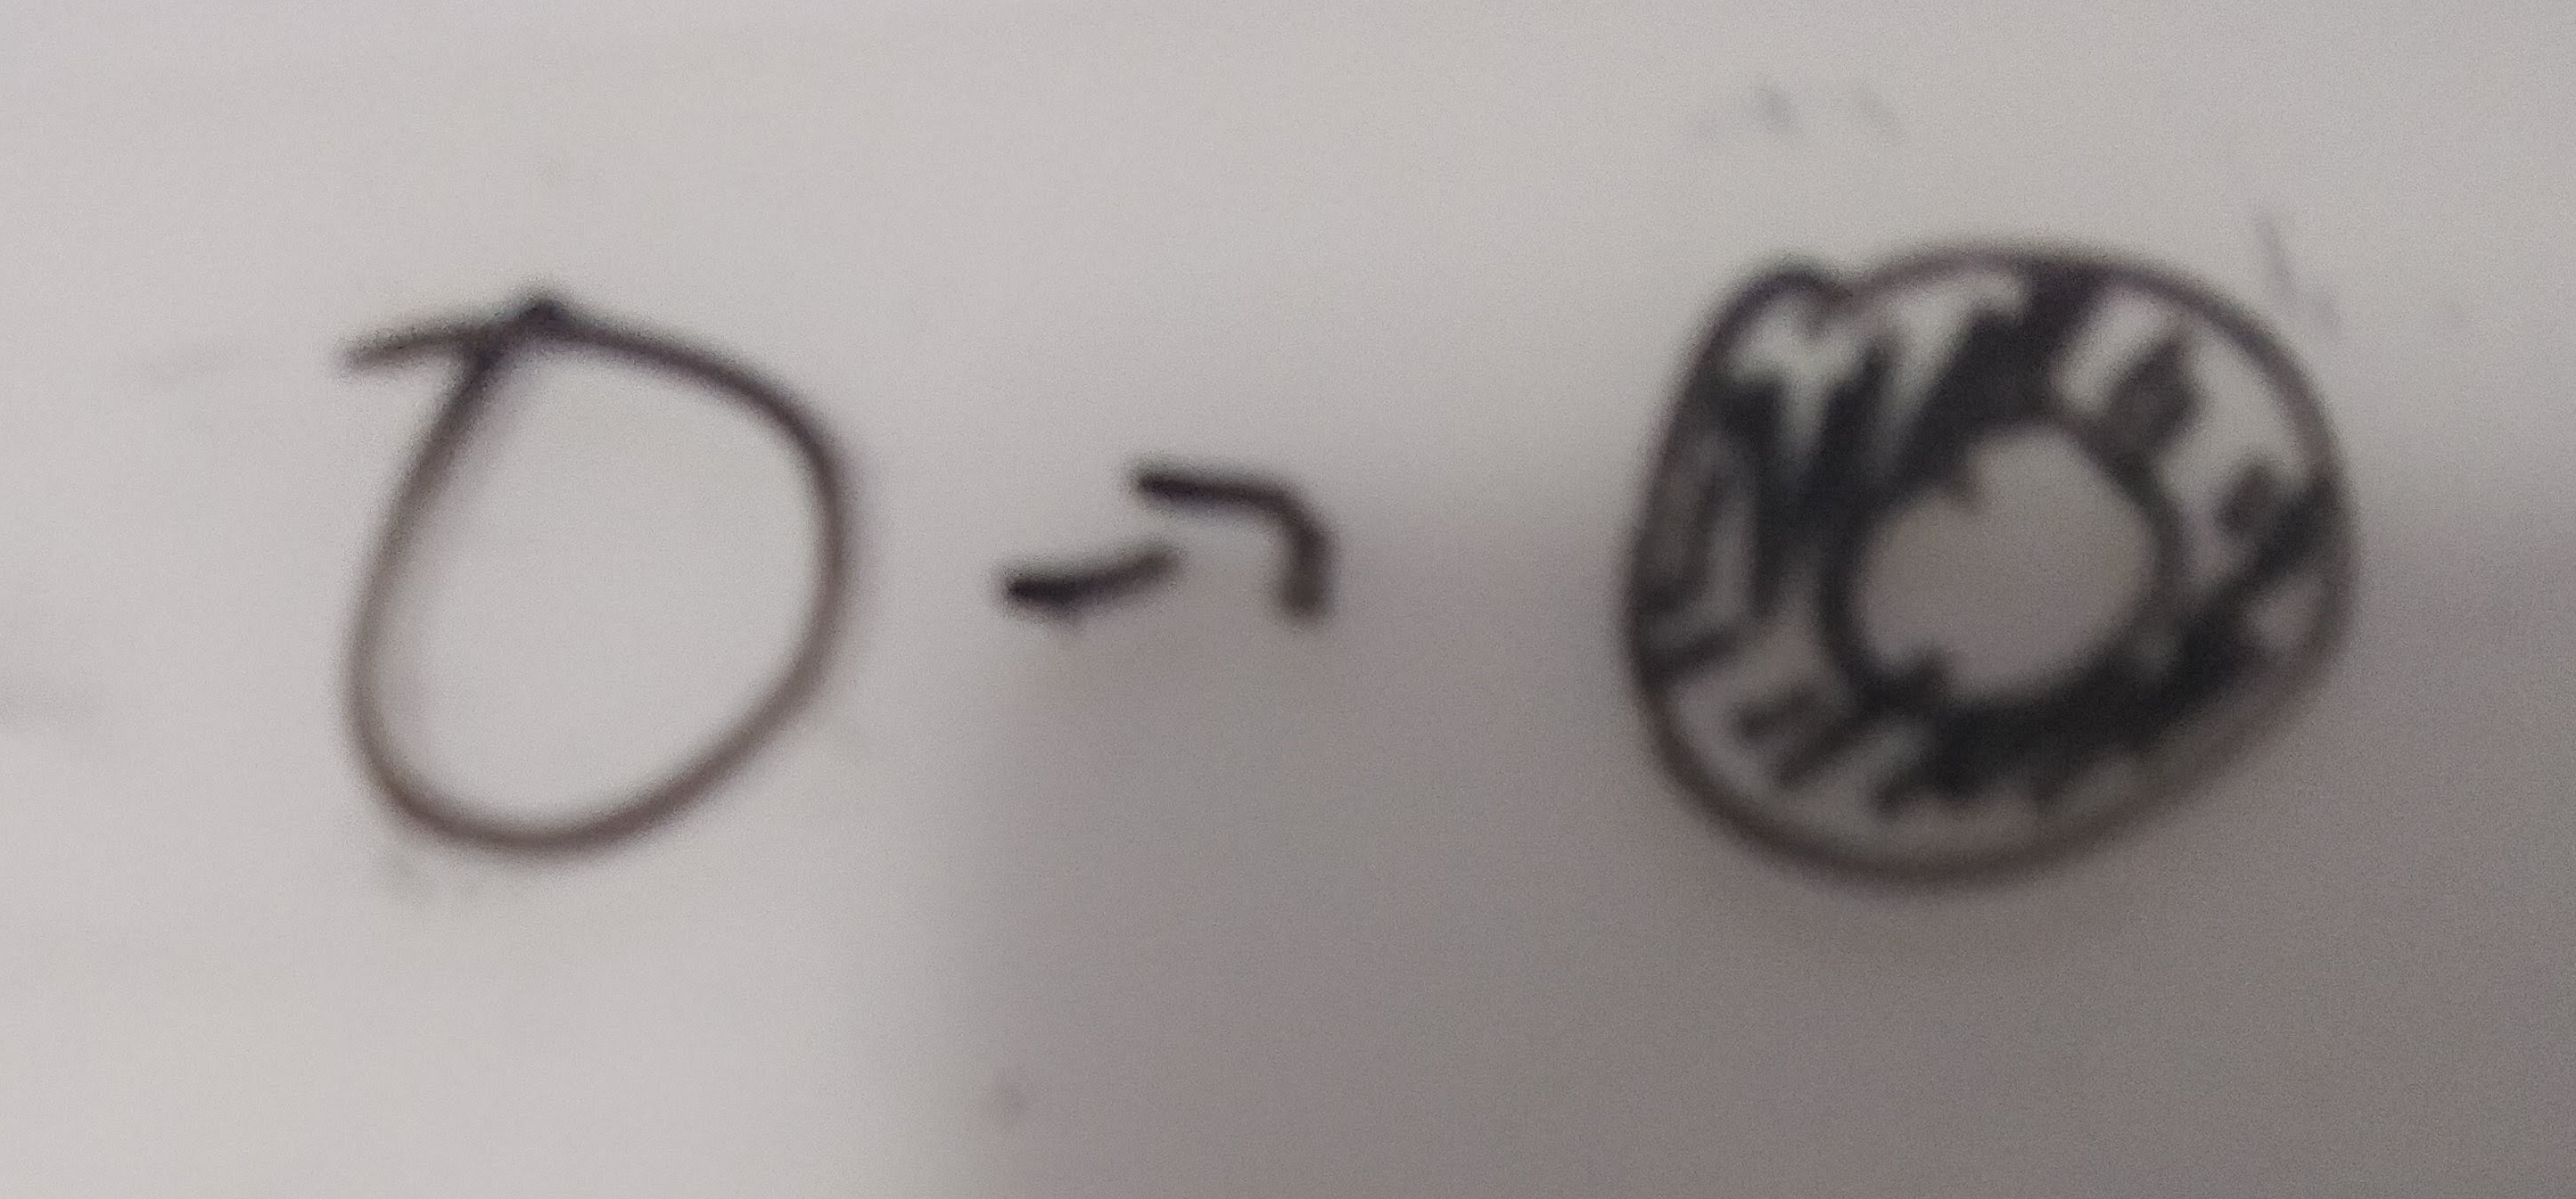
\includegraphics[width=\textwidth]{figures/math/diff_type_q.png}
    \caption{These two glyphs are generated by the same \vmark\ function, but differ in the value of the edge thickness parameter $\vsection_i$. A valid \vmark\ is one where a shift in $\vsection_i$ is reflected in the glyph generated by \gsection.}
    \label{fig:artist_mark_change}
\end{figure}

The glyph in figure~\ref{fig:artist_mark_change} has the following characterstics \vfiber specified by  $(xpos,\, ypos,\, color,\, thickness)$ such that one section is $\vsection=(0,0,0,1)$ and $\vmark(\vsection) = \gsection$ generates a piece of the thin hollow circle. The equivariance constraint on \vmark is that the action $m=(e, e, e, x+2)$, where e is identity, applied to \vsection\ such that $\vsection^{\prime}=(e,e,e,3)$ has an equivalent action on \gsection that causes $\vmark(\vsection^{\prime})$ to be equivalent to the thicker circle in figure~\ref{fig:artist_mark_change}.


We can describe a mark \cite{bertinIIPropertiesGraphic2011,carpendaleVisualRepresentationSemiology} as \vmark\ with input of all the regions \gbasepoint\ that map back to a set of connected components $\dbasepath \subset \dbase$:
\begin{equation}
\dbasepath = \{\dbasepathpoint \in \dbase \text{ s. t. } \exists \gamma \text{ s.t. } \gamma(0)=\dbasepoint \text{ and }\gamma(1)=\dbasepathpoint\}
\end{equation}
where the path\cite{ConnectedSpace2020}  $\gamma$ from \dbasepoint\ to \dbasepathpoint\ is a continuous function from the interval [0,1]. We define the mark as the graphic generated by $\vmark(\gbase_{\dbasepathpoint})$

\begin{equation}
    \begin{tikzcd}
        \gtotal \arrow[r, shift left] & \gbase_\dbasepathpoint \arrow[rr, "\vindex(\gbasepoint)", shift left] \arrow[l, "\gsection(\gbase_\dbasepathpoint)"] &  & \dbasepath_{\dbasepoint} \arrow[ll, "\vindex^{-1}(\dbasepath)"]
        \end{tikzcd}
    \label{eq:mark}
\end{equation}
such that for every mark there is at least one corresponding section on \dbase. We define a glyph as a composite of multiple \vmark\, in keeping with Munzner's definition of the glyph as an object with internal structure arising from multiple marks\cite{munznerVisualizationAnalysisDesign2014}.  

\subsubsection{Sample Graphics \vmark}
In this section we formulate the minimal Q that will generate distinguishable graphical marks: non-overlapping scatter points, a non-infinitely thin line, and a heatmap. 
\begin{figure}[H]
    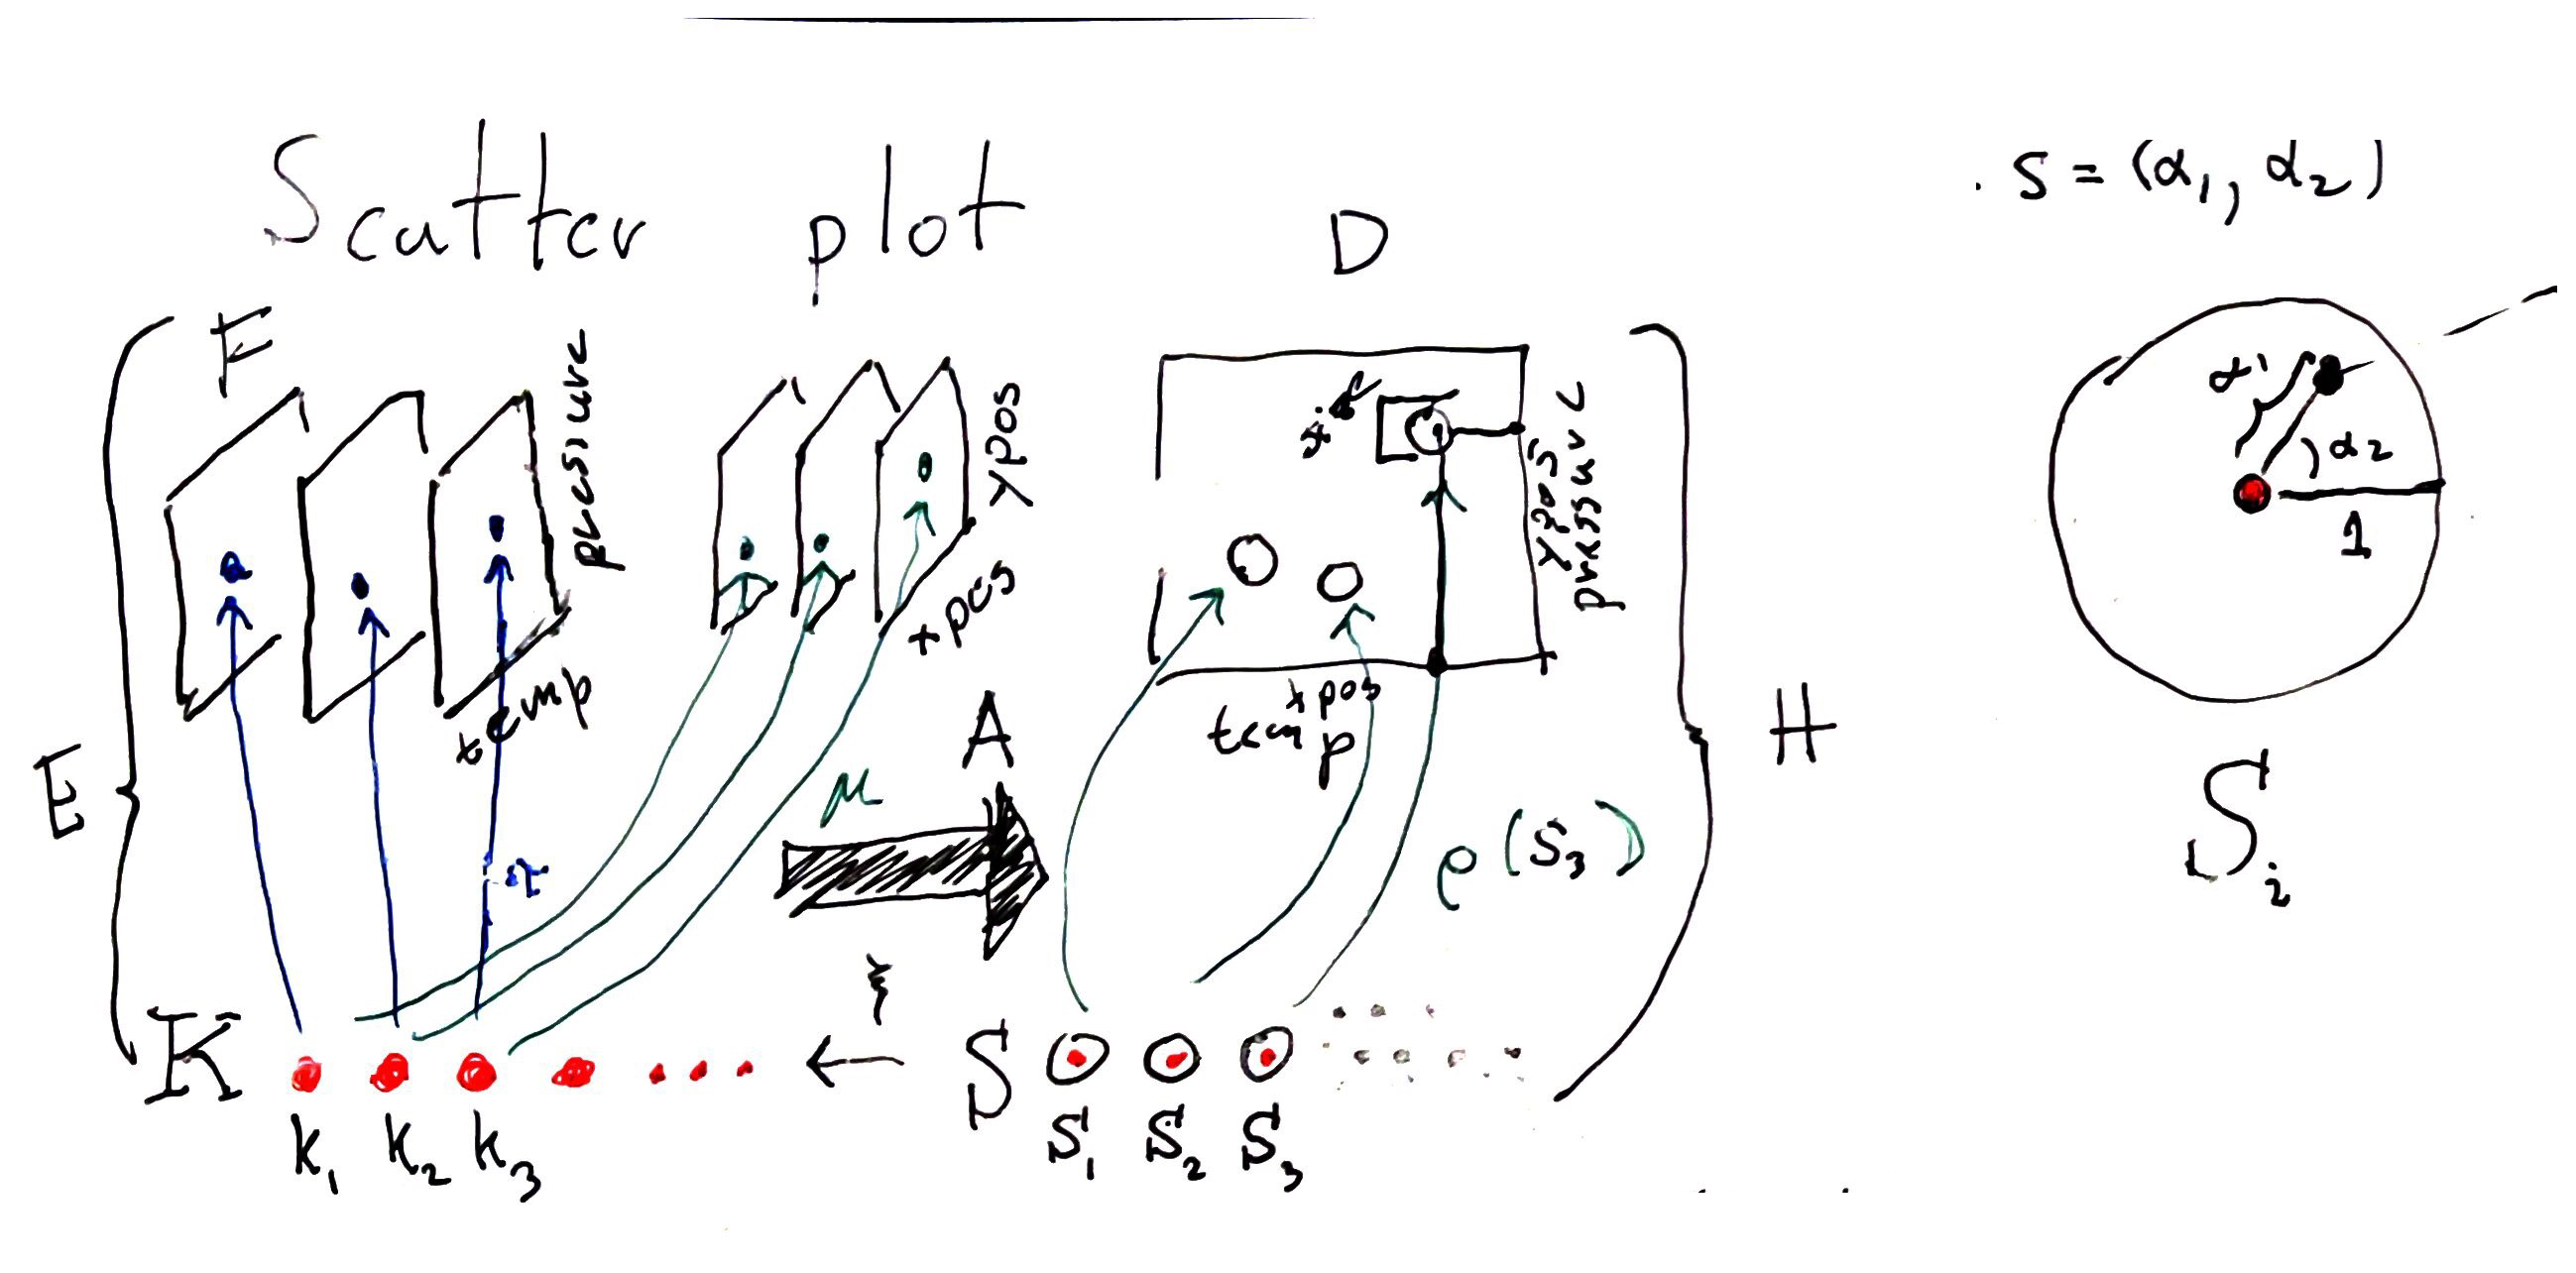
\includegraphics[width=.75\textwidth]{figures/math/scatter.png}
    \caption{The data is discrete points (temperature, time). Via \vchannel\ these are converted to (xpos, ypos) and pulled over discrete \gbase. These values are then used to parameterize \gsection which returns a color based on the parameters (xpos,ypos) and position $\alpha, \beta$ on $\gbase_{\dbasepoint}$ that \gsection\ is evaluated on. 
    }
    \label{fig:artist_scatter}
\end{figure}
The scatter plot in figure~\ref{fig:scatter} can be defined as $\vmark(xpos, ypos)(\alpha, \beta)$ where color $\gsection_{RGB} = (0,0,0)$ is defined as part of \vmark\ and $\gbasepoint=(\alpha, \beta)$ defines the region on \gbase. The position of this swatch of color can be computed relative to the location on the disc $\gbase_{\dbasepoint}$ as shown in figure~\ref{fig:artist_scatter}:
\begin{align}
x &= size\bullet \alpha \bullet \cos(\beta) + xpos\\
y &= size\bullet \alpha \bullet \sin(\beta) + ypos
\end{align}

such that $\gsection(\gbasepoint) = (x, y, 0, 0, 0)$ colors the point (x,y) black.
\begin{figure}[H]
    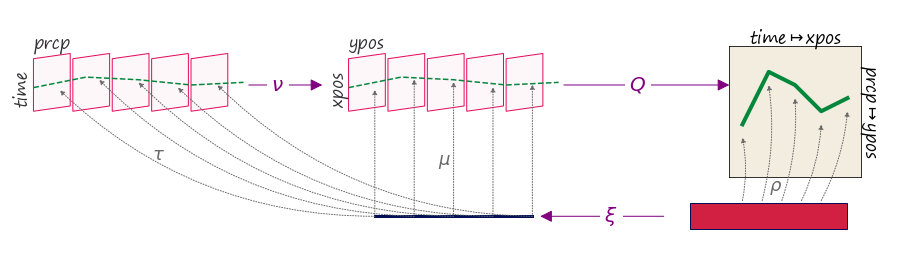
\includegraphics[width=.75\textwidth]{figures/math/line.png}
    \caption{The line fiber $(time,\, temp)$ is thickend with the derivative $(time^{\prime},\, temperature^{\prime}$ because that information will be necessary to figure out the tangent to the point to draw a thick line. This is because the line needs to be pushed perpendicular to the tangent of (xpos, ypos). \note{this is gonna move once this gets regenerated w/ labels} The data is converted to visual characteristics (xpos, ypos). The $\alpha$ coordinates on \gbase\ specifies the position of the line, the $\beta$ coordinate specifies thickness.}
    \label{fig:artist_line}
\end{figure}

The line plot $\vmark(xpos, \hat{n_{1}}, ypos, \hat{n_{2}})(\alpha, \beta)$ shown in fig~\ref{fig:artist_scatter} exemplifies the need for the jet discussed in section~\ref{sec:sheaf_stalk}. The line needs to know the tangent of the data to draw an envelope above and below each (xpos,ypos) such that the line appears to have a thickness. The magnitude of the thickness is 
\begin{equation}
    \lvert n \rvert = \sqrt{{n_{1}}^2 + {n_{2}}^2}
\end{equation}
such that the normal is  
\begin{equation}
    \hat{n_{1}} = \frac{n_1}{\lvert n \rvert}, \; \hat{n_{2}} = \frac{n_2}{\lvert n \rvert}
\end{equation}

which yields components of \gsection
\begin{align}
 x = xpos(\vindex(\alpha)) &+ \beta\hat(n_1)(\vindex(\alpha)) \\
 y = ypos(\vindex(\alpha)) &+ \beta\hat(n_2)(\vindex(\alpha)) 
\end{align}

where (x,y) look up the position $\vindex(\alpha)$ on the data and then apply thickness $\beta$ at that location. 


\begin{figure}[H]
    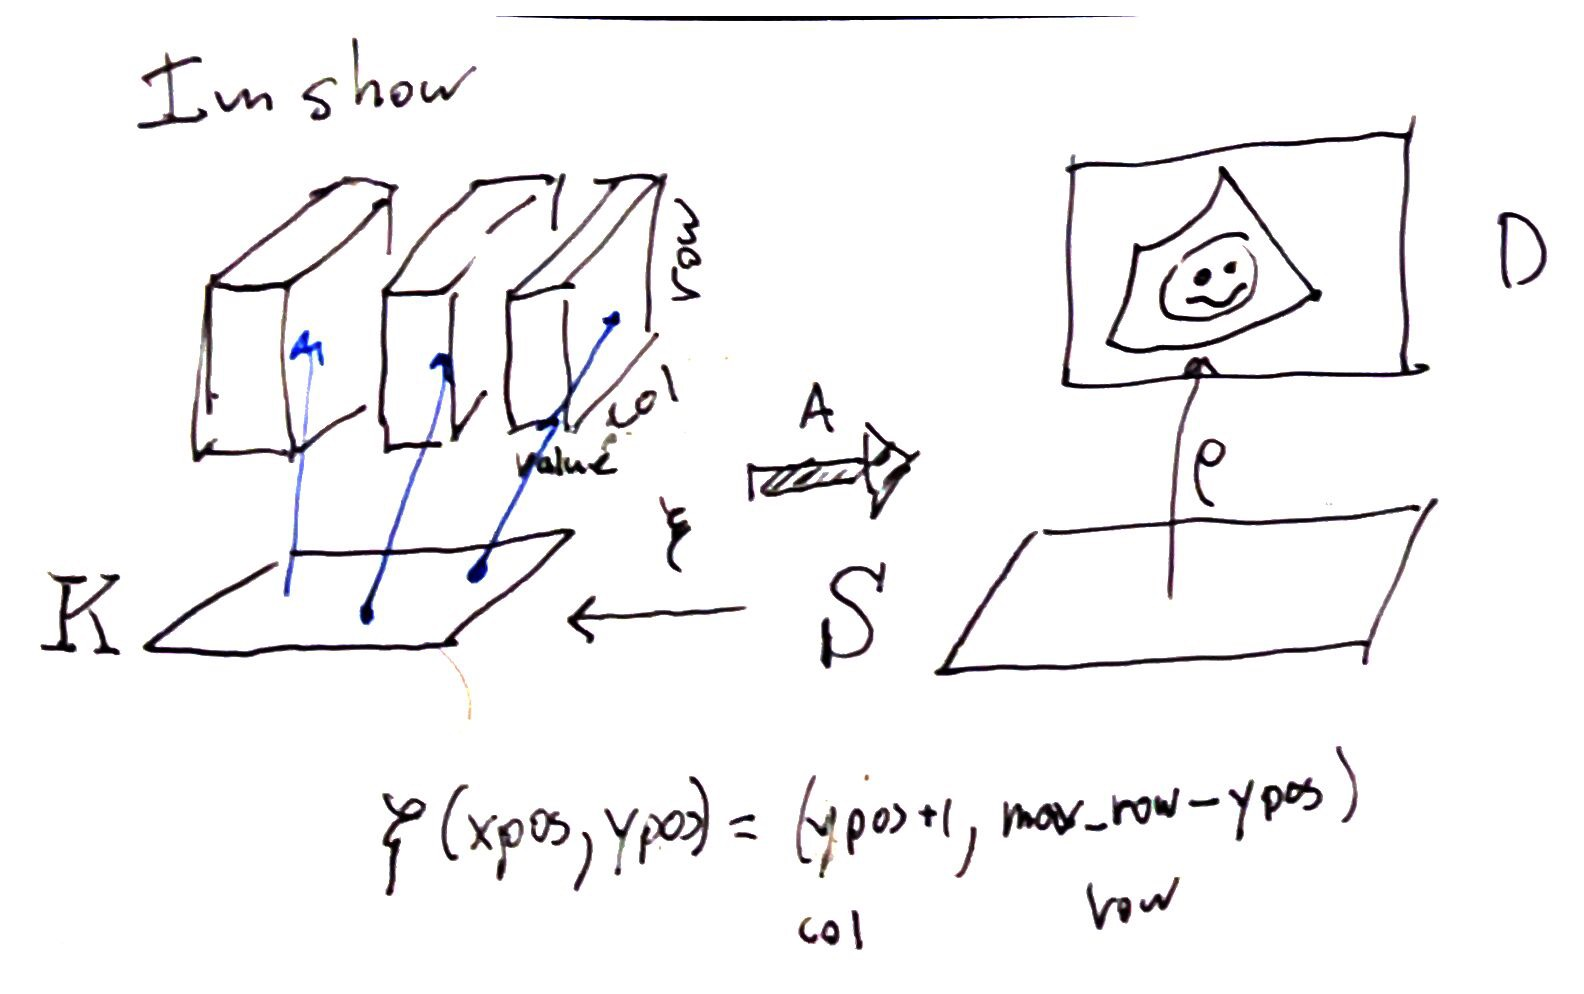
\includegraphics[width=.75\textwidth]{figures/math/heatmap.png}
    \caption{The only visual parameter a heatmap requires is color since \vindex\ encodes the mapping between position in data and position in graphic. }
    \label{fig:artist_heatmap}
\end{figure}

The heatmap $\vmark(color)$ in figure~\ref{fig:artist_heatmap} is a direct lookup $\vindex:\gbase\rightarrow\dbase$ such that 

\begin{align}
R &= R(\vindex(\alpha, \beta))\\
G &= G(\vindex(\alpha, \beta))\\
B &= B(\vindex(\alpha, \beta))
\end{align}
where \vindex\ may do some translating to a convention expected by \vmark\, for example reorientng the array such that the first row in the data is at the bottom of the graphic. 

\subsubsection{Assembly factory \vmarkd}
\begin{figure}
    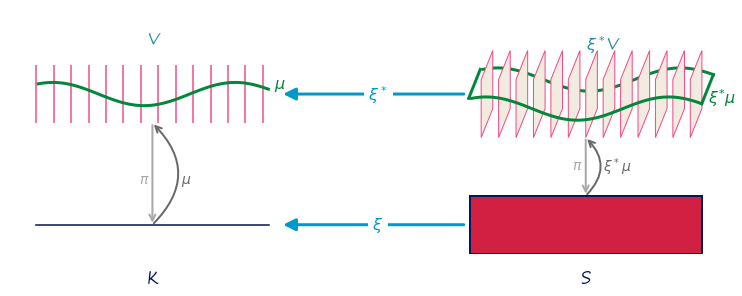
\includegraphics[width=.75\textwidth]{figures/math/q_hat.png}
    \caption{The pullback of the visual bundle \vtotalpull\ is the replication of a \vsection\ over all points \gbasepoint\ that map back to a single \dbasepoint. Because the \vsection\ is the same, we can constract a \vmarkd\ on \vsection\ over \dbasepoint\ that will fabricate the \vmark\ for the equivalent set of \gbasepoint\ associated to that \dbasepoint}
    \label{fig:artist_q_hat}
\end{figure}
As shown in eq~\ref{eq:artist_diagram}, \vmark\ is a bundle map $\vmark: \vtotalpull\rightarrow \gtotal$ where \vtotalpull\ and \gtotal\ are both bundles over \gbase. Because $\vpreimg\ subset \gbase$ such that many \gbasepoint\ go to one \dbasepoint, by definition of the pull back $\vtotalpull \mid_{\vpreimg} = \vpreimg \times \vfiber$. This means that the fiber \vtotal is copied over the preimage in \vpreimg. Given a section \vsectionpull\ pulled back from \vsection\ on $\pi:\vtotal\rightarrow\dbase$ and $\gbasepoint \in \vpreimg$, then the section $\vsectionpull(s) = \vindex^*(\vsection(\dbasepoint))$ is the image of $(\dbasepoint, \vsection(\dbasepoint)) \mapsto (\gbasepoint, \vsectionpull(\gbasepoint))$ for all \gbasepoint\ where $\vindex(\gbasepoint) = \dbasepoint$. This is illustrated in figure~\ref{fig:artist_q_hat}, where a \vsection\ over \dbasepath\ is copied over all  $\vindex(\gbasepoint) = \dbasepoint$. 

When \vmark\ maps sections $\vmark: \Gamma(\vtotalpull) \rightarrow \Gamma(\gtotal)$, if we restrict \vmark\ input to \vsectionpull, then $\vmark(\vsectionpull) = \gsection$ depends on \gbasepoint. This means that $\gsection(\gbasepoint) \coloneqq \vmark(\vsectionpull)(s)$, but since \vsectionpull\ is constant on \vpreimg, we can define a function $\vmarkd(\vsection(k))(s) \coloneqq \vmark((\vsectionpull)(\gbasepoint))$ where $\vpreimg = \dbasepoint$. 

In fact, \vmarkd\ is a map from visual to graphic $\vmarkd:\Gamma(\vtotal) \rightarrow \Gamma(\gtotal)$ locally over \dbasepoint\ such that $\vmarkd:\Gamma(\vtotal_{\dbasepoint}) \rightarrow \Gamma(\gtotal\mid_{\vpreimg})$. This allows us to construct a \vmarkd\ that only depends on \dbase, such that for each $\vsection(\dbasepoint)$ there is part of $\gsection\mid_{\vpreimg}$. The advantage of \vmarkd\ is that \gbase is part of the rendering stage of the pipeline and therefore hidden from the Matplotlib artists and therefore there is no direct way to construct a true \vmark. 

\subsubsection{Composition of Artists: +}
\begin{figure}
    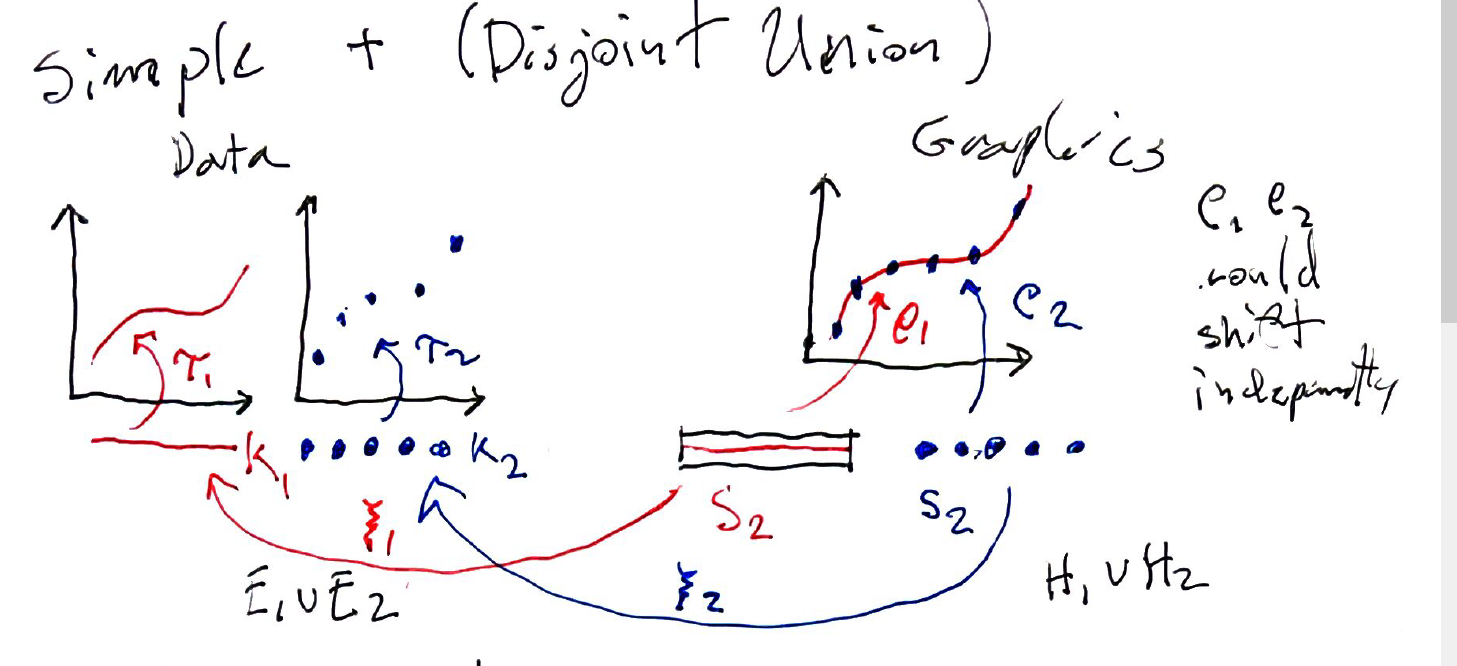
\includegraphics[width=1\textwidth]{figures/math/addition_operator.png}
    \caption{$\dsection_1$ and $\dsection_2$ are distinct datasets passed through artists $\vartist_1$ and $\vartist_2$ to generate graphics $\gsection_1$ and $\gsection_2$. These graphics happen to be rendered to the same image, but otherwise have no intrinsinc link.}
    \label{fig:artist_plus}
\end{figure}
In this paper we define a simple addition operator that is the disjoint union of fiber bundles \dtotal.  For example, in figure~\ref{fig:artist_plus} the scatter plot $\dtotal_1$ and the line plot $\dtotal_2$ have different \dbase that are mapped to seperate \gbase. To fully display both graphics, the composite graphic $\vartist_1 + \vartist_2$ needs to include all records on both $\dbase_1$ and $\dbase_2$, which are the sections on the disjoint union $\dbase_1 \sqcup \dbase_2$. This in turn yields disjoint graphics $\gbase_1 \sqcup \gbase_2$ rendered to the same image. Constraints can be placed on the disjoint union such as that the fiber components need to have the same \vchannel position encodings or that the position \vsection need to be in a specified range. There are situations where $\dbase_2 \hookrightarrow \dbase_1$ that underpin more complex, especially interactive, visualizations; these cases require defining a more complex addition operator that is out of scope for this work. 


\subsubsection{Equivalance class of artists $\vartist^{\prime}$}
\label{sec:artist_equivalance}
As formulated above, every artist function \vartist\ has fixed \vchannel\ and \vmark\ which  generates a distinct graphic \gsection. It is impractical to implement an artist for every single graphic; instead we implement the equivalence class of artists $\{\vartist \in \vartist^{\prime}: \vartist_{1} \equiv \vartist_{2}\}$. Equivalent artists have the same fiber bundle \vtotal\ and same assembly function \vmark\, but act on different sections \vsection. To further simplify implementation, we identify a minimal \vfiber\ associated with each $\vartist^{\prime}$ that defines what visual characteristics of the graphic must originate in the data such that the graphic is identifiable as a given chart type. 

\begin{figure}[H]
    \caption{Each of these graphics is generated by a different artist \vartist which is the equivalance class of scatter plots $\vartist^{\prime}$\note{this is gonna be a whole bunch of scatter plots}}
    \label{fig:artist_equivalence}
\end{figure}
For example, a scatter plot of red circles is the output of one artist, a scatter plot of green squares the output of another, as are the rest of the graphs in figure~\ref{fig:artist_equivalance}. These two artists are equivalent since their only difference is in the literal visual encodings (color, shape). Shape and color could also be defined in \vmark\, but the position must come from the fiber $\vfiber=(xpos,ypos)$ since fundementally a scatter plot is the plotting of one position against another\cite{friendlyBriefHistoryData2008}. We also use this criteria to identify derivative types, for example the bubble chart\cite{tufteVisualDisplayQuantitative2001} is a type of scatter where by definition the glyph size is mapped from the data. 

\subsection{Making the fiber bundle computable}
\label{sec:triangulization}
\begin{figure}[H]
    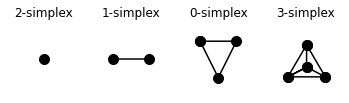
\includegraphics{figures/math/simplex.png}
    \caption{Simplices can encode the connectivity of the data, from fully disconnected (0 simplex) records to all records are connected to at least 3 others}
    \label{fig:triangle_simplex}
\end{figure}
%%big data
One way of expressing the connectivity of records in a dataset is to implement \dbase\ as a simplacial complex, which is a set of simplicies such as those shown in figure~\ref{fig:triangle_simplex}. The advantage of triangulization is that it is general enough to work for more complex topology based visualization methods \cite{heineSurveyTopologybasedMethods2016} while also providing a consistent interface of vertices, edges, and faces for \vindex\ to map into. When triangulated, the simplices encode the continuity in the data

\begin{table}[H]
    \begin{center}
        \begin{tabular}{|l|l|l|}\hline
        \textbf{simplex} & \textbf{continuity} & \textbf{\dsection}   \\ \hline
        vertex  & discrete   & \dsection(\dbasepoint)                  \\ \hline
        edge    & 1D         & $\dsection(\dbasepoint,\, \alpha)$        \\ \hline
        face    & 2D         & $\dsection(\dbasepoint,\, \alpha,\, \beta)$\\ \hline
        \end{tabular}
        \caption{}
        \label{tab:triangulization}
    \end{center}
\end{table}

such that each section is bound to a simplex $\dbasepoint \in \dbase$. As shown in table~\ref{tab:triangulization}, in a 1D continuous spaces each \dsection\ lies distance $\alpha$ along edge \dbasepoint, while in a 2D continuous space each \dsection\ lies at coordinate $\alpha, \beta$ on the face \dbasepoint. This is directly analogous to indexing to express connectivity in N-D arrays, while also natively supporting graphs and trees as they are simplacial complices of nodes and edges. Path connected components are then sections where edges or faces meet. 

\begin{figure}[H]
    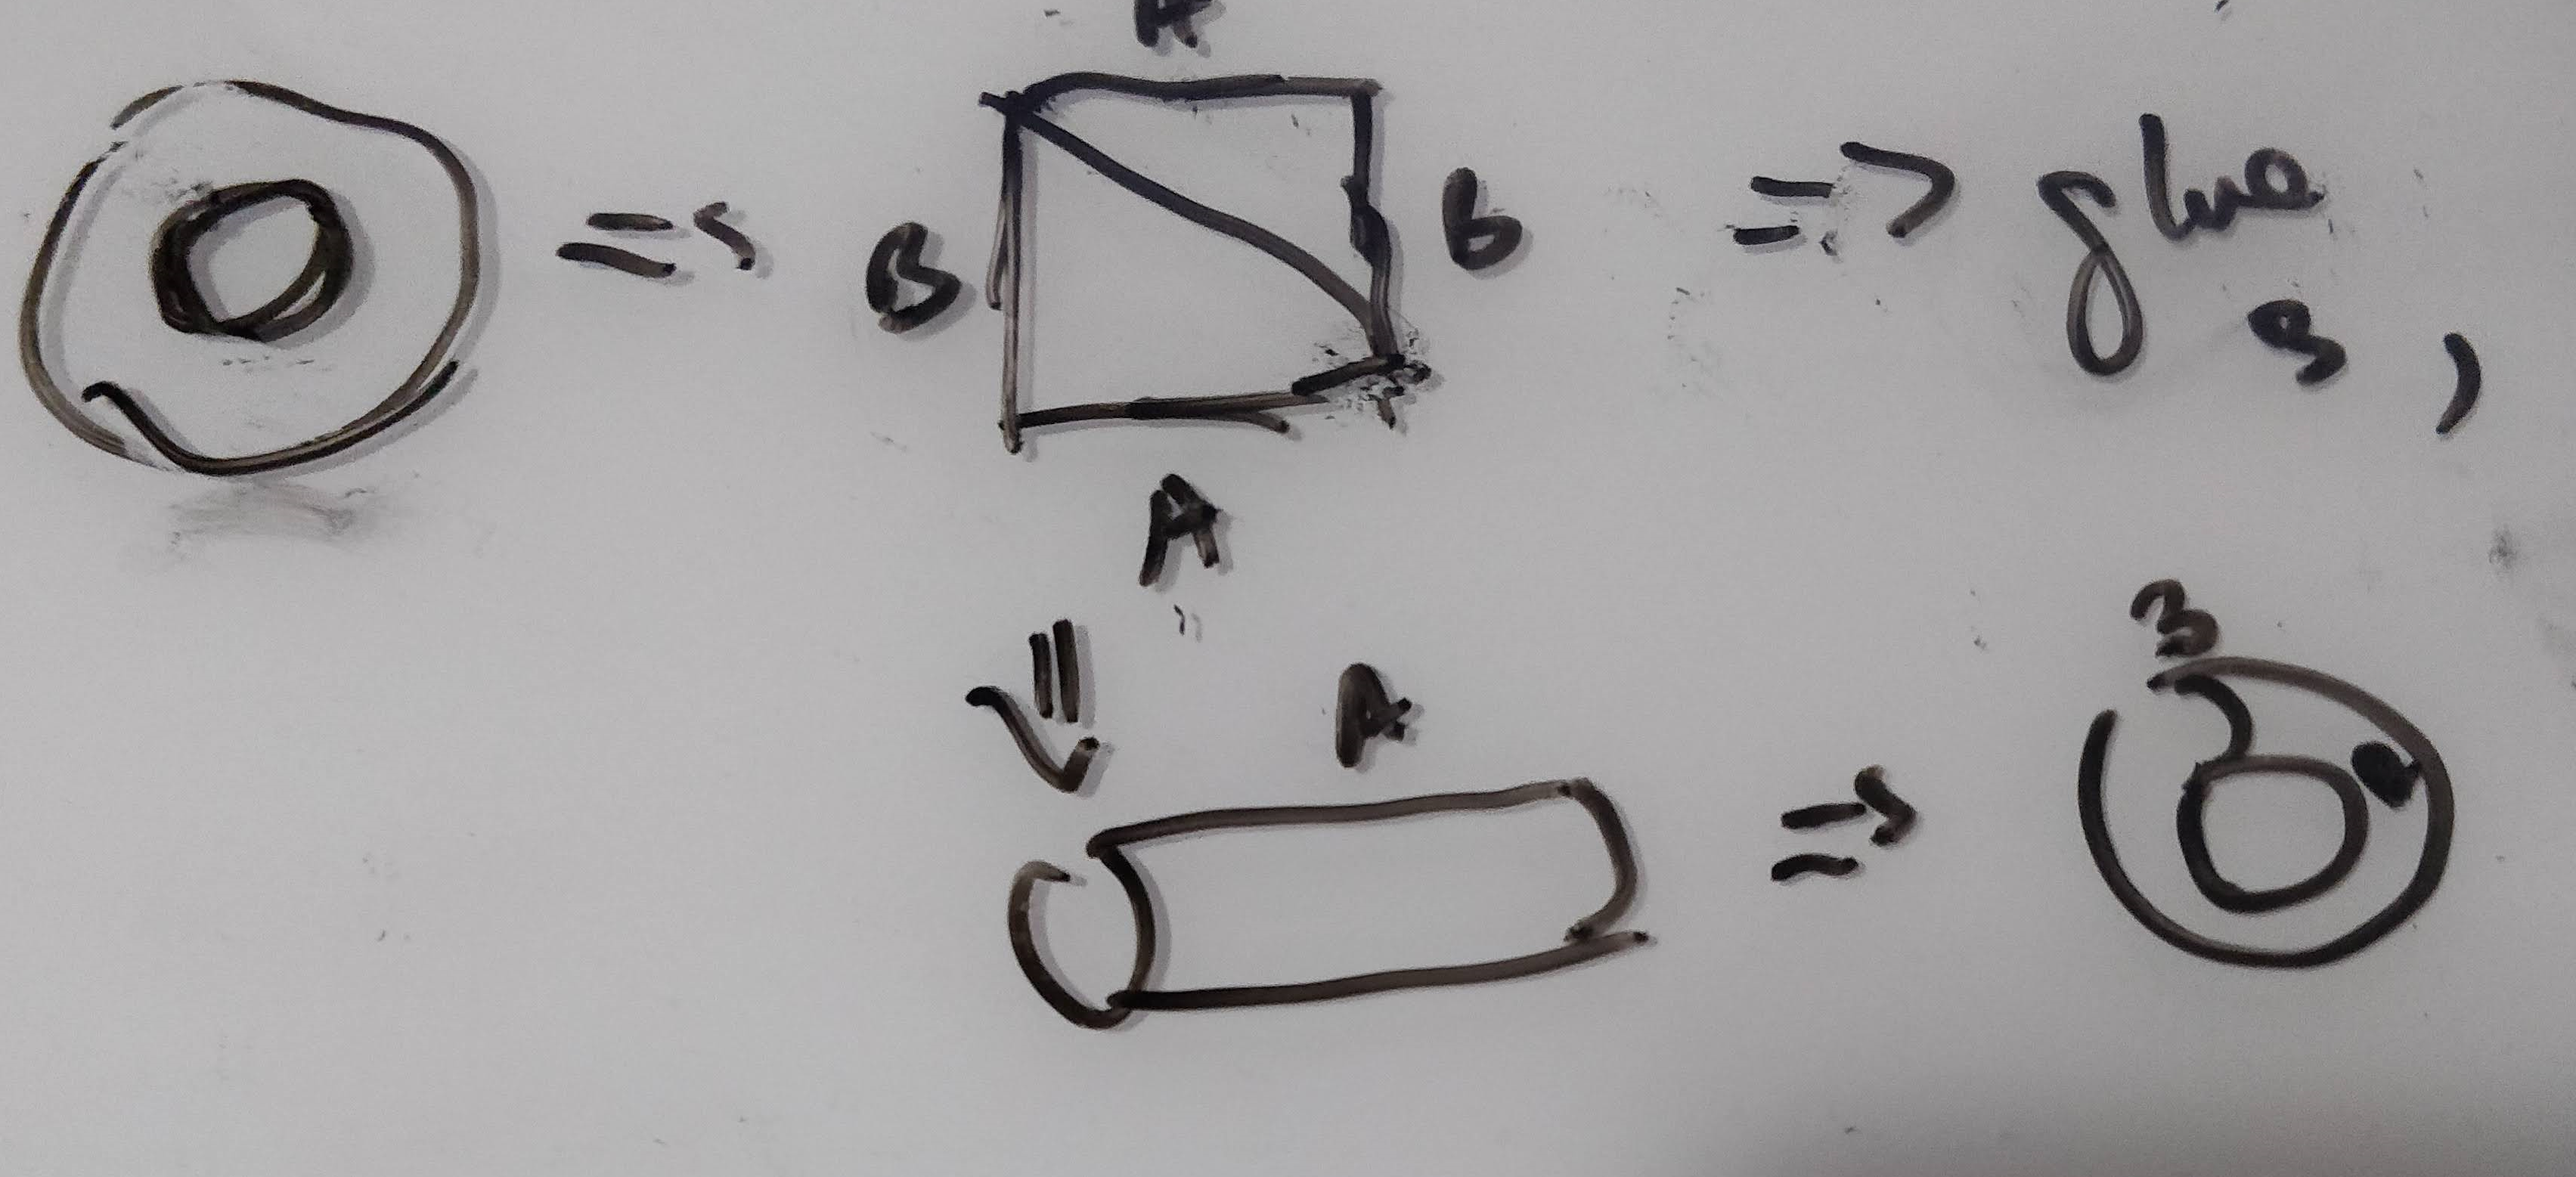
\includegraphics[width=\textwidth]{figures/math/triangle_torus.png}
    \caption{The torus \dtotal is unraveled into a simplacial complex of 2 faces \dbase. Transition functions are defined on the edges of \dbase such that surface can be glued back into the torus.
    \note{add cross sections a and b to ring and color same as edges in complex}}
    \label{fig:triangle_torus}
\end{figure}
One way of encoding the torus in figure~\ref{fig:triangle_torus} while retaining the continuity of both cross sections $a, b$ is to unravel it into a simplacial complex of two triangles with labeled edges. Transition functions $\delta$ are defined on the edges such that $a$ can be glued to $a^\prime$ and $b$ to $b^\prime$ to reconstruct the torus. This simplacial complex is then used as the base space encoding the continuity of data that lies in the torus. A constraint on the transition functions is that the monoid actions on the fibers on the edges of \dtotal\ are commutative $\monoid*\dfiber\mapsto \delta(\monoid\dfiber)= \monoid*\delta(\dfiber)$

\begin{figure}[H]
    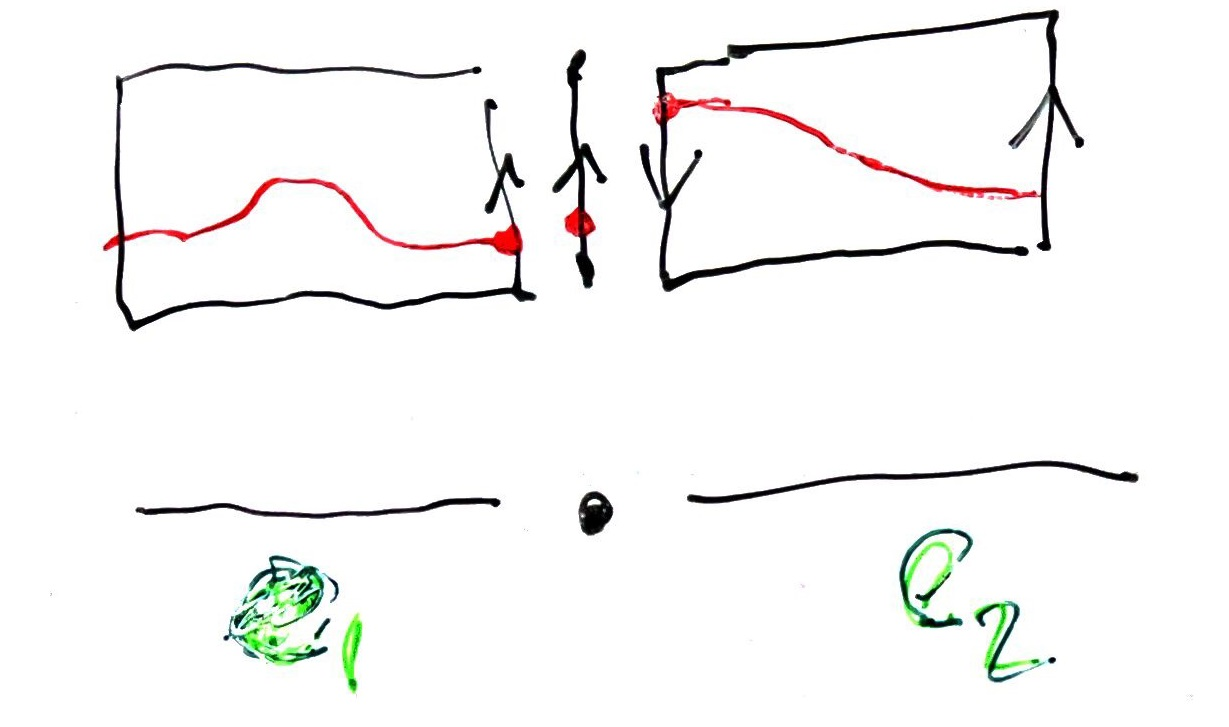
\includegraphics[width=\textwidth]{figures/math/transition_functions.png}
    \caption{Many non-trivial spaces can be made locally trivial by dividing \dtotal into locally trivial subspaces and defining transition functions between the edges on \dbase for how to glue the two subspaces such that the \dsection are continuous.}
    \label{fig:data_base_transition}
\end{figure}
Another advantages of triangulization is that it provides a way to encode non-trivial structures such as the mobius strip\cite{MobiusStripNLab}. As shown in figure ~\ref{fig:data_base_transition}, one way of making the mobius strip trivial is to seperate it into two spaces $\dtotal_1$ and $\dtotal_2$ and then define transition functions that specify that the edges of $\dtotal_1$ need to be reversed to line up with $\dtotal_2$ such that the sections along the edges meet. As with the torus, the transition functions must preserve monoid commutativity. 

\end{document}